\documentclass[aps,prb,onecolumn,10pt,floatfix,superscriptaddress]{article} %pueden consultarse mas clases en 'REVTEX 4.1 Command and Options Summary'
%prb es la revista con las citas como superindices
%document class: article [twocolums,10pt,a4paper], book

\usepackage{listings}
\usepackage{amssymb} %amssymb y amsmath se usan juntos para ampliar
\usepackage{amsmath} %la cantidad de simbolos disponibles

\usepackage{graphicx} % permite usar imagenes fuera del modo dvi
\usepackage[spanish]{babel} % le dice al compilador que el idioma de escritura es espa\~nol
\usepackage[latin1]{inputenc} % permite usar caracteres de idiomas derivados del lat\'in
% \usepackage[T1]{fontenc} % permite usar acentos en el c\'odigo fuente

 \usepackage[pdftex,colorlinks=true,pdfstartview=FitH,linkcolor=blue,citecolor=blue,urlcolor=blue]{hyperref} % agrega hiperv\'inculos a la presentaci\'on en pdf

\usepackage[left=3cm,right=3cm,top=2cm,bottom=2cm]{geometry}
\renewcommand{\thefootnote}{\fnsymbol{footnote}}
%\usepackage[switch]{lineno} %Marca el n\'umero de linea... Poner \linenumbers donde se quiere empezar a contar
%\DeclareGraphicsExtensions{.pdf,.png,.jpg,.eps}%lo obvio

\begin{document}

\title{Pr\'actica $4$ : Aprendizaje supervisado en redes multicapa.}

\author{Melisa Maidana Capit\'an}

\date{Junio 2013} % se puede utilizar \today para que ponga autom\'aticamente la fecha

\maketitle 
%\tableofcontents
% 

\setlength{\parindent}{30pt}
\setlength{\parskip}{2.5ex plus 0ex minus 0ex}

\section*{Resumen}

Se programaron diferentes arquitecturas para entrenar una red neuronal para aprender la regla XOR y para aprender el mapeo log\'istico. En el primer caso, se compararon las velocidades de aprendizaje para diferentes arquitecturas y cantidad de neuronas de entrada. El el segundo caso, se verific\'o la capacidad de generalizaci\'on de la red, es decir, de resolver un problema que no fue aprendido.

Para programar estas redes se utiliz\'o el algoritmo de retroprogaci\'on.

\section{Aprendizaje supervisado}

En los problemas de memorias asociativas, los pesos de las conexiones son medianamente determinados a partir de reglas simples como la de Hebb. Sin embargo, a veces resulta pr\'actico adoptar formas iterativas, que permitan determinar los valores de los pesos mejorando los mismos paso a paso. Este es el proceso conocido como aprendizaje.

Existen dos tipos de aprendizaje para una red neuronal, supervisado y no supervisado. En el aprendizaje supervisado, la salida se compara con la respuesta esperada o "correcta" y es realimentada con el error cometido. Mientras que en el aprendizaje no supervisado no hay salidas correctas o incorrectas, si no que la red debe aprender sola a descubrir caracter\'isticas interesantes en las entradas.

En general, en aprendizaje supervisado se entrena la red con un conjunto de pares de entrada-salida que concuerdan. Se dice que la red puede generalizar el aprendizaje cuando se le presenta un par entrada-salida que no se encuentra en su lista de entrenamiento, y la misma puede encontrar los pesos apropiados para obtener exitosamente la salida deseada.

Se denomina perceptr\'on a una red que tiene una capa de entrada ($\xi$) y una de salida ($\zeta$), sin capas ocultas. Un algoritmo para lograr el aprendizaje en este tipo de redes es el "feed-forward". Un problema puede resolverse por medio de una red representada por un perceptr\'on simple, si es mismo es linearmente separable. Esta limitaci\'on se aplicaci\'on del perceptr\'on no se aplica a redes con capas ocultas. La importancia de las redes multicapa radica en su capacidad de aprendizaje utilizando algoritmos "back-propagation".

El algoritmo "back-propagation" da una regla para modificar los pesos de cualquier red "feed-forward" para aprender un conjunto de pares entrada-salida de entrenamiento.

\subsection{Algoritmo de retropropagaci\'on en redes con una capa oculta}

Dada una red de dos capas, se denomina $O_i$ a la salida de la i-\'esima neurona, $V_{j}$ al valor de las neuronas de la capa oculta, $\xi_{k}$ a los valores de las neuronas en la capa de entrada. Adem\'as se donomina $J_{jk}$ a los pesos que conectan la capa de entrada con la oculta, y $W_{ij}$ a los pesos de las conexiones entre la capa oculta y la salida.

La entrada puede tomar valores $\xi^{\mu}_{k}$ con $k=1...N$ y $\mu=1...p$, donde $p$ es el n\'umero de patrones y $N$ el n\'umero de neuronas de la capa de entrada.

Dado un patr\'on $\mu$, la unidad $j$ de la capa oculta recibe una entrada dada por 

\begin{equation}
h^{\mu}_{j} = \sum_{k} J_{jk} \xi^{\mu}_{k}
\end{equation}

y produce una salida $V^{\mu}_{j} = g(h^{\mu}_{j})$, donde $g$ es generalmente una funci\'on no lineal.

La i-\'esima unidad de salida recibe

\begin{equation}
h^{\mu}_{i} = \sum_{j} W_{ij} V^{\mu}_{j} = \sum_{j} W_{ij} g(\sum_{k} J_{ij} \xi^{\mu}_{k})
\end{equation}

y produce una salida $O^{\mu}_{i} = g(h^{\mu}_{i})$.

Los valores de umbrales pueden considerarse agregando una neurona a la capa de entrada con valor seteado en $-1$ y conectada a todas las neuronas de la red.

El error o funci\'on de costo se define como 

\begin{equation}
E = \frac{1}{2} \sum_{\mu i} (\xi^{\mu}_{i}-O^{\mu}_{i})^{2}
\end{equation}

Y las reglas de adaptaci\'on de los pesos entra la capa de salida y la oculta est\'an dadas por

\begin{equation}
\Delta W{ij} = \eta \sum_{\mu} \delta^{\mu}_{i} V^{\mu}_{j}
\end{equation}

donde $\delta^{\mu}_{i} = g'(h^{\mu}_{i}) (\zeta^{\mu}_{i}-O^{\mu}_{i})$ y $\eta$ es la tasa de aprendizaje. Y entra la capa oculta y la de entrada 

\begin{equation}
\Delta J_{jk} = \eta \sum_{\mu} \delta^{\mu}_{j} \xi^{\mu}_{k}
\end{equation}

donde $\delta^{\mu}_{j} = g'(h^{\mu}_{j}) \sum_{i} W_{ij} \delta^{\mu}_{i}$.

En este informe se utiliz\'o una funci\'on de transferencia no lineal $g(x) = tanh (x)$.

\section{Arquitecturas y algor\'itmos para aprender XOR.}

\subsection{Algortimo de retropropagaci\'on para aprender XOR:Redes con dos neuronas de entrada}

Dadas dos arquitecturas neuronales diferentes, se utiliz\'o el algoritmo de retropropagaci\'on para aprender el XOR. En la Fig.(\ref{arq1}) se muestran las arquitecturas utilizadas para aprender el XOR.

\pagebreak

%==FIGURA======FIGURA======FIGURA======FIGURA======FIGURA======FIGURA=====
\begin{figure}[!htd] 
   	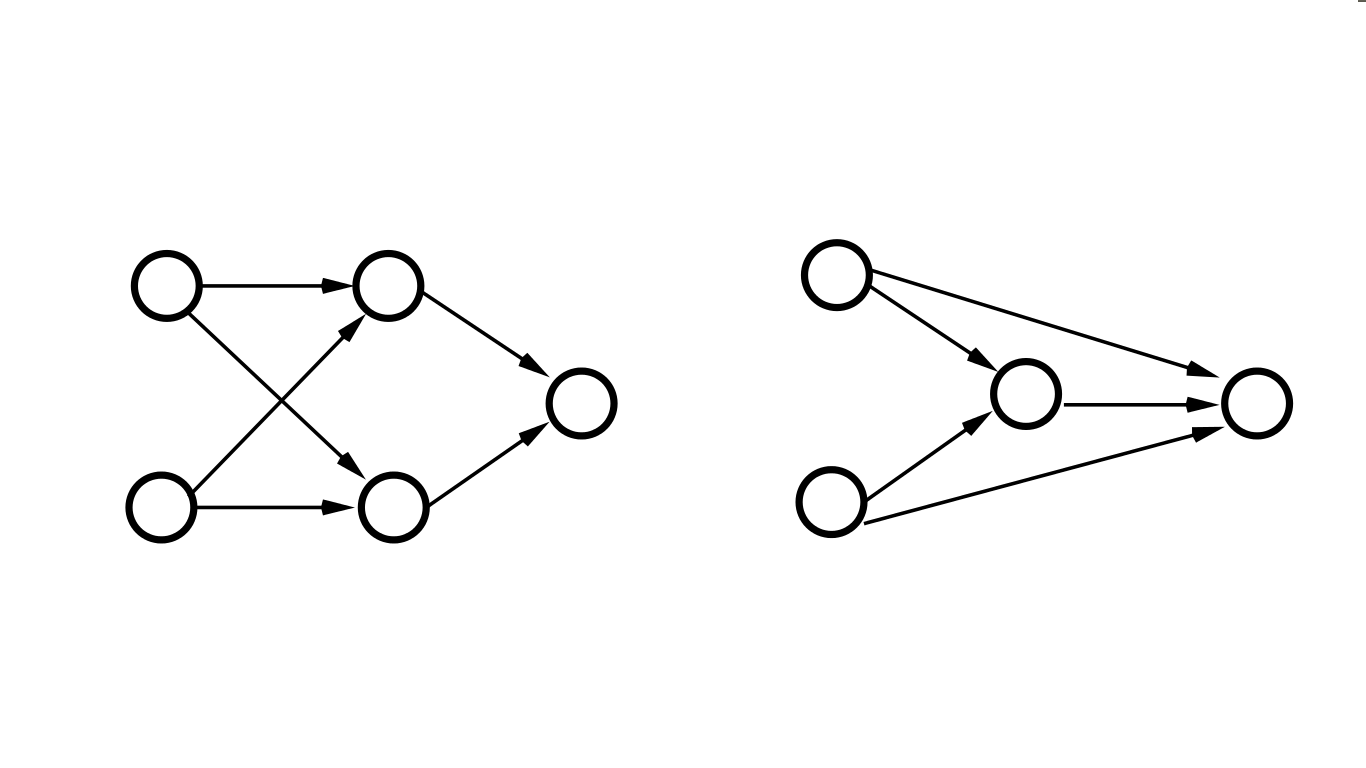
\includegraphics[scale=0.25 ]{xor.png}
   	\begin{center}
  \caption{\label{arq1} Arquitecturas utilizadas para aprender XOR. A las mismas se les agreg\'o una neurona de entrada que representa los umbrales.}
     	    \end{center}
 \end{figure}
%==FIGURA======FIGURA======FIGURA======FIGURA======FIGURA======FIGURA=====

Para ambas arquitecturas se calculo el tiempo de convergencia, definido como el n\'umero de iteraciones necesarias para que la red aprenda a dar una salida correcta a los patrones de entrada.

%==FIGURA======FIGURA======FIGURA======FIGURA======FIGURA======FIGURA=====
\begin{figure}[!htd] 
	\begin{minipage}[b]{0.450\linewidth}
   	    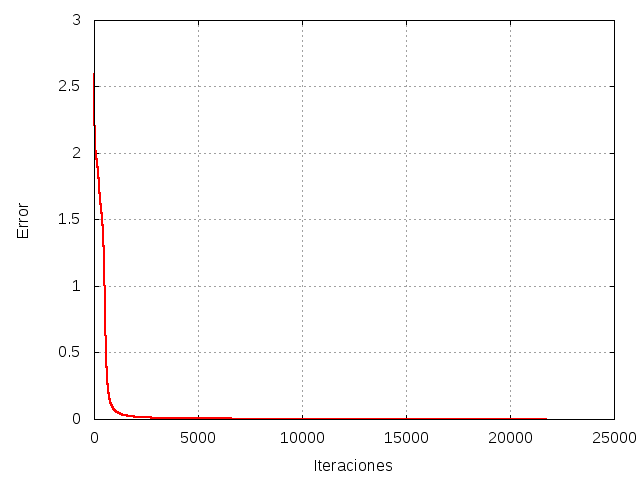
\includegraphics[scale=0.32 ]{xor1.png}
   	    \begin{center}
  \caption{\label{error1a} Error como funci\'on del n\'umero de iteraciones para la arquitectura de la Fig.(\ref{arq1}).}
     	    \end{center}
   \end{minipage}
   \begin{minipage}[b]{0.450\linewidth}
   	    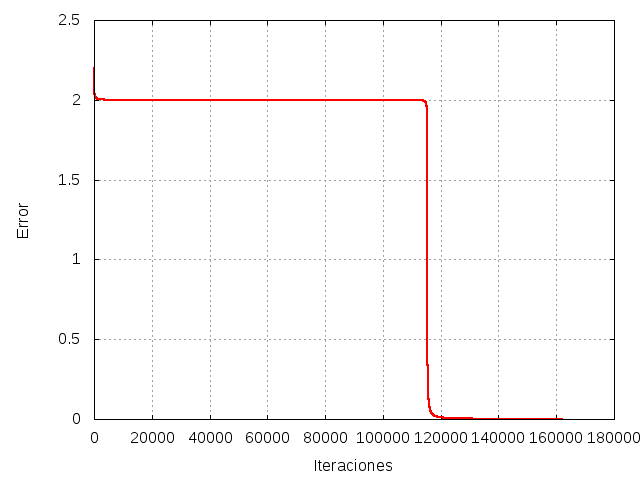
\includegraphics[scale=0.32 ]{xor2.png}
   	     \begin{center}
  \caption{\label{error1b}  Error como funci\'on del n\'umero de iteraciones para la arquitectura de la Fig.(\ref{arq2}).}
     	    \end{center}
   \end{minipage} 
 \end{figure}
%==FIGURA======FIGURA======FIGURA======FIGURA======FIGURA======FIGURA=====

Se observa que la red con mayor cantidad de neuronas en la capa oculta, aprende m\'as r\'apido. Es decir, el error entre la salida deseada y la salida de la red disminute m\'as rapidamente con el n\'umero de iteraciones.

La red entrenada consiste en que la misma tenga los pesos apreopiados para resolver todos los patrones aprendidos. Si llamamos $i$ a las neuronas de entrada, $j$ a las de oculta y $k$ a las de la capa salida, y $J_{ij}$ son los pesos de la capa de entrada hacia la oculta, $W_{ij}$ a los pesos de la capa oculta hacia la de salida. Llamamos $U1_{j}$ a los umbrales de la capa de entrada a la oculta, y $U2_{k}$ a los umbrales de la campa de entrada a la de salida. 

Entonces, los pesos que se obtuvieron para la red $1$ son $J_11 = 1.47, J_{12} = 1.48, J_{21} = 1.77, J_{22} = 1.81$, $W_{11}=-2.61 , W_{12} = 2.59$, $U1_{1} = -1.28 , U1_{2} = 1.68$ y $U2 = -2.32$.

Entonces, los pesos que se obtuvieron para la red $1$ son $J_11 = 2.19, J_{12} = 2.19$, $W_{11}=4.67$, $U1_{1} =2.19$ y $U2 =-2.27$.

\subsection{Algortimo de retropropagaci\'on para aprender XOR: Redes con N neuronas de entrada y N' neuronas en la capa oculta}

Se generaliz\'o el problema de aprendizaje de XOR a una red con N neuronas en la capa de entrada, N' neuronas en la capa oculta y una neurona en la capa de salida. La generalizaci\'on consiste en que la salida es el producto de las N entradas.

%==FIGURA======FIGURA======FIGURA======FIGURA======FIGURA======FIGURA=====
\begin{figure}[!htd]
\begin{center}
 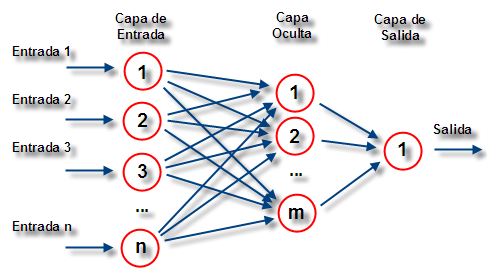
\includegraphics[scale=0.5]{red3.png}
  \caption{\label{arq3}}
  \end{center}
 \end{figure}
%==FIGURA======FIGURA======FIGURA======FIGURA======FIGURA======FIGURA=====

Se utilizar\'on distintos valores de N y N' y se calcul\'o el tiempo de convergencia para cada uno. La Fig.(\ref{error3}) muestra el error como funci\'on del n\'umero de iteraciones para diferentes valores de N y N'.

%==FIGURA======FIGURA======FIGURA======FIGURA======FIGURA======FIGURA=====
\begin{figure}[!htd]
\begin{center}
 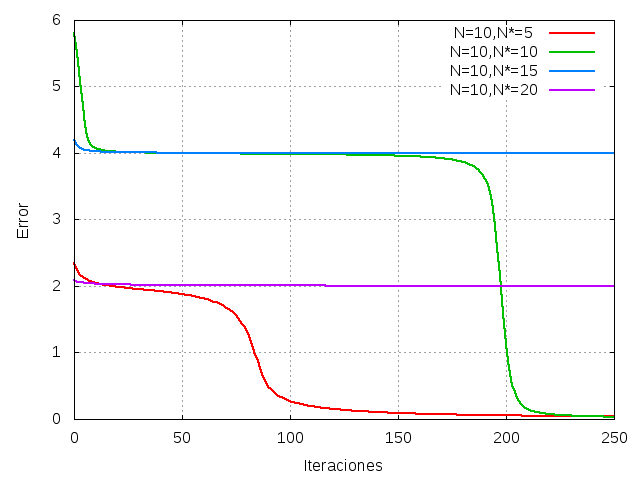
\includegraphics[scale=0.35]{xor3.png}
  \caption{\label{error3} Error como funci\'on de la iteraci\'on para diferentes relaciones entre el n\'umero de neuronas de entrada y el n\'umero de neuronas de la capa oculta.}
  \end{center}
 \end{figure}
%==FIGURA======FIGURA======FIGURA======FIGURA======FIGURA======FIGURA=====

En la Fig.(\ref{error3}) se observa que para valores de $N' < N$ el error no disminuye, por lo que la red tarda m\'as en aprender el problema planteado. Este resultado no tiene mucho sentido, porque en realidad en un problema de redes multicapa, se mapea el problema de la capa de entrada hacia las capas ocultas. Si la dimensi\'on de las capas ocultas es menor que la dimensi\'on de la capa de entrada, el mapeo reduce las dimensiones del problema, por lo que se dificulta el aprendizaje. No pudo encontrarse el error en este programa, pero si se resalta que el resultado no est\'a teniendo mucho sentido.

\section{Algoritmo de retropropagaci\'on para aprender mapeo log\'isto}

Se program\'o la red que presenta la Fig.(\ref{red3}) para aprender el mapeo log\'istico: $x = 4 x (1-x)$.

\pagebreak

%==FIGURA======FIGURA======FIGURA======FIGURA======FIGURA======FIGURA=====
\begin{figure}[!htd]
\begin{center}
 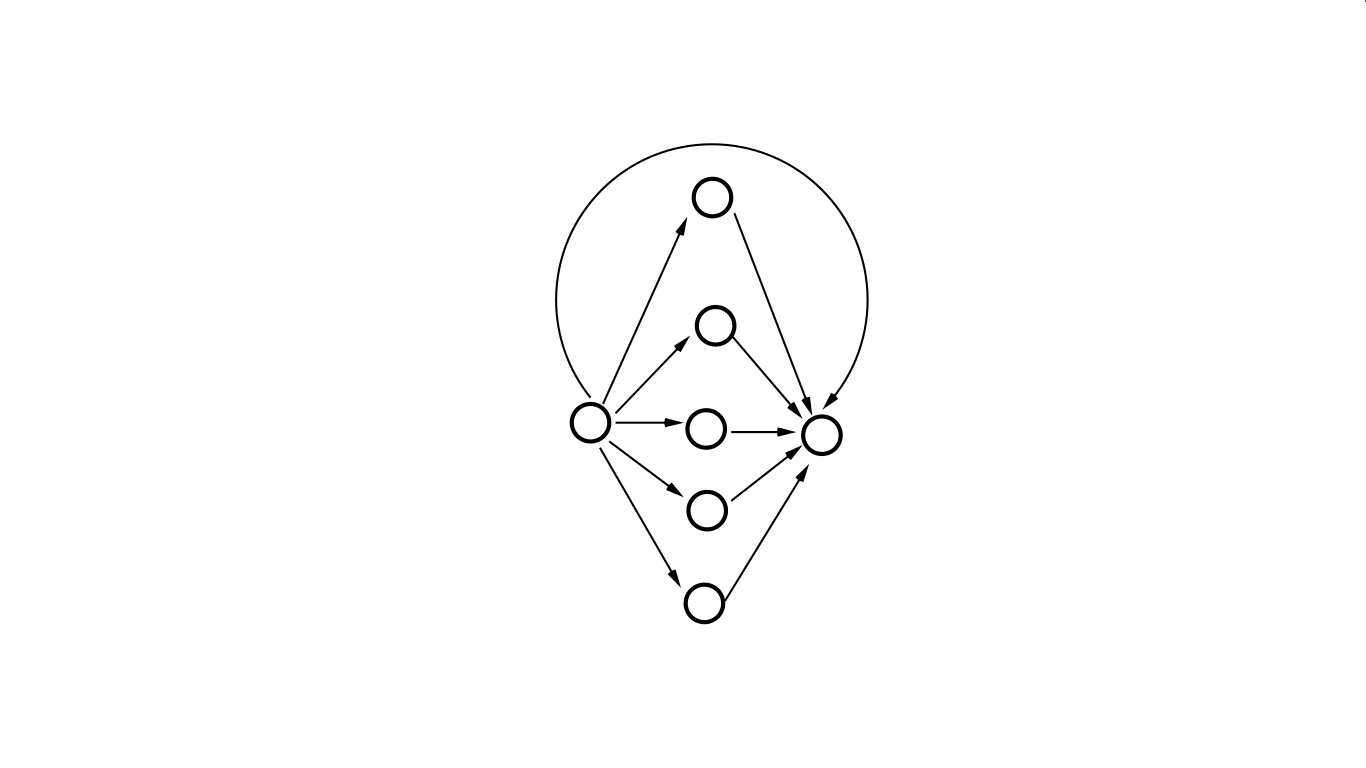
\includegraphics[scale=0.25]{red4.png}
  \caption{\label{red3} Arquitectura utilizada para aprender el mapeo log\'istico.}
  \end{center}
 \end{figure}
%==FIGURA======FIGURA======FIGURA======FIGURA======FIGURA======FIGURA=====

Una vez aprendido el mapeo log\'istico, se verific\'o que la red pueda generalizar. Es decir, la capacidad de dar una respuesta correcta ante patrones que no fueron aprendidos.

La Fig.(\ref{mapeo}) presenta los resultados para los patrones aprendidos y y la Fig.(\ref{general})para la generalizaci\'on.
%==FIGURA======FIGURA======FIGURA======FIGURA======FIGURA======FIGURA=====
\begin{figure}[!htd] 
	\begin{minipage}[b]{0.450\linewidth}
   	    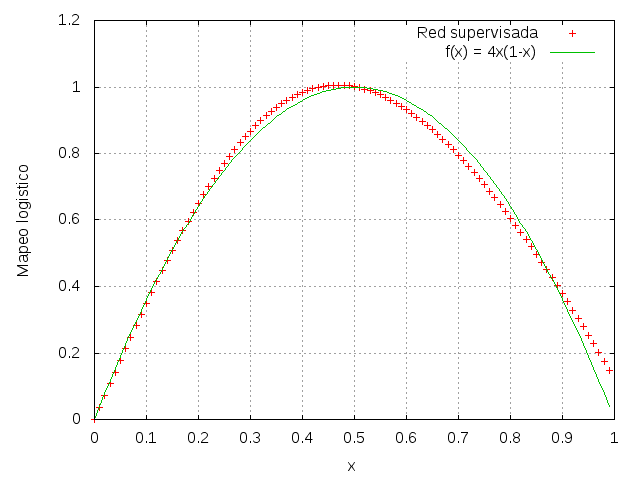
\includegraphics[scale=0.32 ]{logistico.png}
   	    \begin{center}
  \caption{\label{mapeo} Aprendizaje de la red para $100$ patrones equidistantes en el intervalo $[0,1]$.}
     	    \end{center}
   \end{minipage}
   \begin{minipage}[b]{0.450\linewidth}
   	    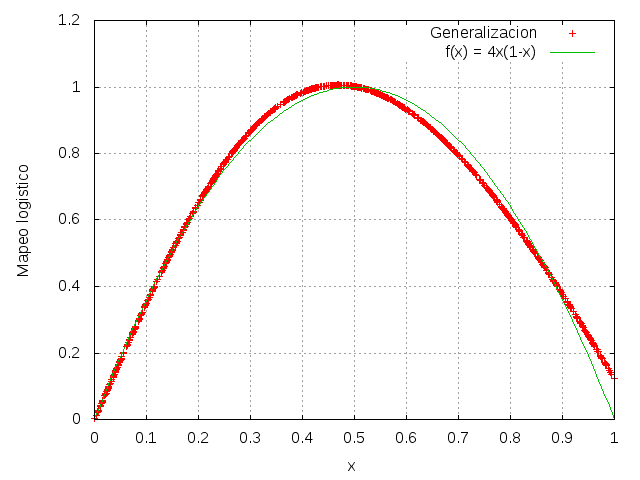
\includegraphics[scale=0.32 ]{generaliza.png}
   	     \begin{center}
  \caption{\label{general} Presentaci\'on de $1000$ valores aleatorios en el intervalo $[0,1]$.}
     	    \end{center}
   \end{minipage} 
 \end{figure}
%==FIGURA======FIGURA======FIGURA======FIGURA======FIGURA======FIGURA=====

La Fig.(\ref{error_log}) muestra la curva del error en el aprendizaje como funci\'on de las iteraciones cuando se le presentan $100$ patrones.

%==FIGURA======FIGURA======FIGURA======FIGURA======FIGURA======FIGURA=====
\begin{figure}[!htd]
\begin{center}
 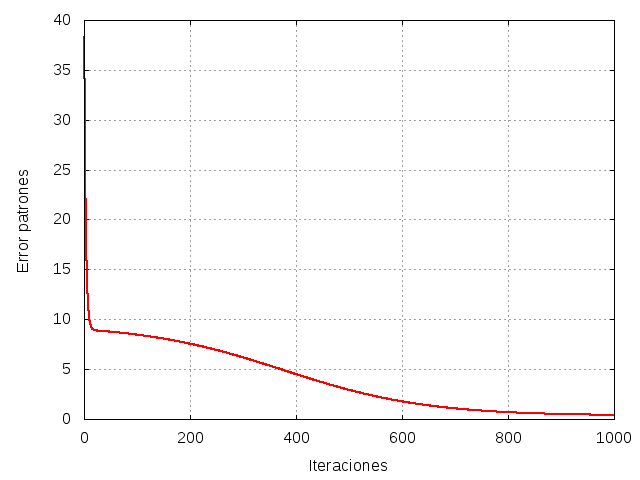
\includegraphics[scale=0.4]{error_log.png}
  \caption{\label{error_log} Curva de error en el aprendizaje del mapeo log\'istico.}
  \end{center}
 \end{figure}
%==FIGURA======FIGURA======FIGURA======FIGURA======FIGURA======FIGURA=====


Podemos calcular el error de aprendizaje como

\begin{equation}
E_{apren} = \frac{1}{2} \frac{1}{P} \sum^{P}_{i=1} [\zeta_{i} - o_{i}]^{2}
\end{equation}

donde $P$ es el n\'umero de patrones presentados a la red para el aprendizaje. Y podemos calcular el error de generalizaci\'on como 

\begin{equation}
E_{gral} = \frac{1}{2} \frac{1}{G} \sum^{G}_{i=1} [\zeta_{i} - o_{i}]^{2}
\end{equation}

donde $G$ es el n\'umero de entradas que se le presentaron luego del aprendizaje.

Para un conjunto de $100$ patrones equidistantes en el intervalo $[0,1]$, se obtuvo un error de aprendizaje final $E_{apren} = 0.00049$, y para un conjunto de $1000$ puntos elegidos al azar en el mismo intervalo (distintos a los patrones) se obtuvo $E_{gral} = 0.00050$.


\section{Programas en C}

\subsection{Algoritmo para aprender XOR: Redes con $2$ entradas}

\begin{lstlisting}[frame=single,breaklines=true]

void InitWeigh(MatDoub &matrix);
void XOR_patrones(MatDoub &matrix);
	
#define N_IN 2
#define N_HIDE1 2
#define N_OUT 1
#define P 4
#define eta 0.01

int main(){
	
MatDoub patrones(P,N_IN);
MatDoub J(N_HIDE1,N_IN),W(N_OUT,N_HIDE1);
VecDoub umbral1(N_HIDE1);
double umbral2;
int estado_umbral=-1;
double salida_deseada,o;
VecDoub v(N_HIDE1);	
double error,delta;
VecDoub delta2(N_HIDE1);

srand(time(0));
	
InitWeigh(J);
InitWeigh(W);
for(int i=0;i<N_HIDE1;i++)
	umbral1=rand()*1.0/RAND_MAX;
umbral2 = rand()*1.0/RAND_MAX;
XOR_patrones(patrones);

double error_global=1;
int it=0;
	while(error_global>0.001){
		error_global=0;
		for(int i=0;i<P;i++){
			salida_deseada=patrones[i][0]*patrones[i][1];
			
			for(int k=0;k<N_HIDE1;k++){
				v[k]=0;
				for(int j=0;j<N_IN;j++)
					v[k]+=J[k][j]*patrones[i][j];
				v[k]+=umbral1[k]*estado_umbral;		
				v[k]=tanh(v[k]);
				}
			o=0;	
			for(int k=0;k<N_HIDE1;k++)
				o+=W[0][k]*v[k];
			o+=umbral2*estado_umbral;
			o=tanh(o);
			//cout << salida_deseada << " " << o << endl;
			error = 0.5*(salida_deseada-o)*(salida_deseada-o);	
			error_global+=error;
			delta = (salida_deseada-o)*(1-o*o);

			for(int k=0;k<N_HIDE1;k++)
				delta2[k]=delta*W[0][k]*(1-v[k]*v[k]);

			for(int k=0;k<N_HIDE1;k++)
				W[0][k]+=eta*delta*v[k];	
			umbral2+=eta*delta*estado_umbral;	

			for(int k=0;k<N_HIDE1;k++){
				for(int j=0;j<N_IN;j++)
					J[k][j]+=eta*delta2[k]*patrones[i][j];
				umbral1[k]+=eta*delta2[k]*estado_umbral;
				}
			}
		//cout << it << " " << error_global << endl;
		it++;
		}
return 0;
}

void InitWeigh(MatDoub &matrix){
	
int n = matrix.nrows();
int m = matrix.ncols();
	
for(int i=0;i<n;i++){
	for(int j=0;j<m;j++){
		matrix[i][j] = rand()*1.0/RAND_MAX;
		}
	}
}

void XOR_patrones(MatDoub &matrix){
	
int n = matrix.nrows();
int m = matrix.ncols();
	
matrix[0][0]=1;
matrix[0][1]=1;
matrix[1][0]=-1;
matrix[1][1]=-1;
matrix[2][0]=1;
matrix[2][1]=-1;
matrix[3][0]=-1;
matrix[3][1]=1;
	
}

\end{lstlisting}

Las modificaciones que suguiere el ejercicio $1.b$ se implementaron en el mismo algoritmo presentado anteriormente de la siguiente manera.

\begin{lstlisting}[frame=single,breaklines=true]

for(int k=0;k<N_HIDE1;k++)
	o+=W[0][k]*v[k];
for(int j=0;j<N_IN;j++)
	o+=W[0][N_HIDE1+j]*patrones[i][j];
o+=umbral2*estado_umbral;
o=tanh(o);
\end{lstlisting}

\begin{lstlisting}[frame=single,breaklines=true]
for(int k=0;k<N_HIDE1;k++)
	W[0][k]+=eta*delta*v[k];
for(int j=0;j<N_IN;j++)
	W[0][N_HIDE1+j]+=eta*delta*patrones[i][j];
umbral2+=eta*delta*estado_umbral;
\end{lstlisting}

\subsection{Algoritmo para aprender XOR: Redes con $N$ entradas}

\begin{lstlisting}[frame=single,breaklines=true]
void InitWeigh(MatDoub &matrix);
void GeneraPatrones(MatDoub &matrix);
	
int main(){

	int N_IN,N_HIDE1,N_OUT,P;
	printf("Escriba el numero de neuronas de entrada.\n");
	scanf("%d",&N_IN);
	printf("Escriba el numero de neuronas de la capa oculta.\n");
	scanf("%d",&N_HIDE1);
	printf("Escriba el numero neuronas de salida\n");
	scanf("%d",&N_OUT);
	printf("Escriba el numero de patrones\n");
	scanf("%d",&P);
	
	FILE *archivo1,*archivo2;
	string output1=to_string("error_xor")+to_string("_")+to_string(N_IN)+to_string("_")+to_string(N_HIDE1)+to_string(".dat");
	if((archivo1 = fopen(output1.c_str(), "w")) == NULL){
            printf("No puedo abrir el archivo %s.\n", output1.c_str());
            exit(1);
        }
        
	string output2=to_string("salidas_xor")+to_string("_")+to_string(N_IN)+to_string("_")+to_string(N_HIDE1)+to_string(".dat");
	if((archivo2 = fopen(output2.c_str(), "w")) == NULL){
            printf("No puedo abrir el archivo %s.\n", output1.c_str());
            exit(1);
        }
     
    double eta = 0.01;   
	MatDoub patrones(P,N_IN);
	MatDoub J(N_HIDE1,N_IN),W(N_OUT,N_HIDE1);
	VecDoub umbral1(N_HIDE1);
	double umbral2;
	int estado_umbral=-1;
	double o;
	VecDoub v(N_HIDE1);	
	double error,delta;
	VecDoub delta2(N_HIDE1);

	srand(time(0));
	
	InitWeigh(J);
	InitWeigh(W);
	for(int i=0;i<N_HIDE1;i++)
		umbral1=rand()*1.0/RAND_MAX;
	umbral2 = rand()*1.0/RAND_MAX;
	GeneraPatrones(patrones);
	VecDoub salida_deseada(P);
	for(int i=0;i<P;i++){
		double prod=1;
		for(int j=0;j<N_IN;j++){
			prod=prod*patrones[i][j];
			}
		salida_deseada[i]=prod;
		}

	double error_global=1;
	int it=0;
	while(error_global>0.001){
		error_global=0;
		for(int i=0;i<P;i++){
			for(int k=0;k<N_HIDE1;k++){
				v[k]=0;
				for(int j=0;j<N_IN;j++)
					v[k]+=J[k][j]*patrones[i][j];
				v[k]+=umbral1[k]*estado_umbral;		
				v[k]=tanh(v[k]);
				}
			o=0;	
			for(int k=0;k<N_HIDE1;k++)
				o+=W[0][k]*v[k];
			o+=umbral2*estado_umbral;
			o=tanh(o);
			cout << salida_deseada[i] << " " << o << endl;
			error = 0.5*(salida_deseada[i]-o)*(salida_deseada[i]-o);	
			error_global+=error;
			delta = (salida_deseada[i]-o)*(1-o*o);

			for(int k=0;k<N_HIDE1;k++)
				delta2[k]=delta*W[0][k]*(1-v[k]*v[k]);

			for(int k=0;k<N_HIDE1;k++)
				W[0][k]+=eta*delta*v[k];	
			umbral2+=eta*delta*estado_umbral;	

			for(int k=0;k<N_HIDE1;k++){
				for(int j=0;j<N_IN;j++)
					J[k][j]+=eta*delta2[k]*patrones[i][j];
				umbral1[k]+=eta*delta2[k]*estado_umbral;
				}
			}
		fprintf(archivo1,"%i\t%lf\n",it,error_global);
		it++;
		}
		
	for(int i=0;i<N_HIDE1;i++){
		for(int j=0;j<N_IN;j++)
			fprintf(archivo2,"%lf\n",J[i][j]);
		fprintf(archivo2,"%lf\n",umbral1[i]);
		}
	
	for(int i=0;i<N_OUT;i++){
		for(int j=0;j<N_HIDE1;j++)
			fprintf(archivo2,"%lf\n",W[i][j]);
		fprintf(archivo2,"%lf\n",umbral2);
		}
		
	return 0;
	}

void InitWeigh(MatDoub &matrix){
	
	int n = matrix.nrows();
	int m = matrix.ncols();
	
	for(int i=0;i<n;i++){
		for(int j=0;j<m;j++){
			matrix[i][j] = rand()*1.0/RAND_MAX;
			}
		}
	}

		
void GeneraPatrones(MatDoub &matrix){
	
	int n = matrix.nrows();
	int m = matrix.ncols();
	
	double aleatorio;
	for(int i=0;i<n;i++){
		for(int j=0;j<m;j++){
			matrix[i][j]=1;
			aleatorio = rand()*1./RAND_MAX;
			if(aleatorio < 0.5)
				matrix[i][j] = -1;
			}
		}
	}
\end{lstlisting}

\subsection{Algoritmo para aprender mapeo log\'istico}

\begin{lstlisting}[frame=single,breaklines=true]
int main(){
	
	int N_IN=1,N_HIDE1=5,N_OUT=1,P=100;
	/*printf("Escriba el numero de neuronas de entrada.\n");
	scanf("%d",&N_IN);
	printf("Escriba el numero de neuronas de la capa oculta.\n");
	scanf("%d",&N_HIDE1);
	printf("Escriba el numero neuronas de salida\n");
	scanf("%d",&N_OUT);
	printf("Escriba el numero de patrones\n");
	scanf("%d",&P);*/
	
	double eta = 0.001;
	
	VecDoub J(N_HIDE1),W(N_HIDE1);
	double umbral,deltaumbral;
	VecDoub salida_deseada(P);
	VecDoub z(P),o(P);
	VecDoub v(N_HIDE1),delta2(N_HIDE1);
	double delta1;
	
	srand(time(0));
	
	for(int i=0;i<N_HIDE1;i++){
		J[i]=rand()*1.0/RAND_MAX;
		W[i]=rand()*1.0/RAND_MAX;		
		}
	umbral = rand()*1.0/RAND_MAX;
	for(int k=0;k<P;k++)
		z[k]=k*1.0/P;

	double error_patrones=1;
	int it=0;
	while(error_patrones > 0.05){
		error_patrones=0;
		for(int k=0;k<P;k++){	
			salida_deseada[k] = 4*z[k]*(1-z[k]);
			for(int i=0;i<N_HIDE1;i++)
				v[i]=tanh(J[i]*z[k]);
		
			o[k]=umbral*z[k];	
			for(int i=0;i<N_HIDE1;i++)
				o[k]+=W[i]*v[i];			
			
			delta1 = (salida_deseada[k]-o[k]);
			for(int i=0;i<N_HIDE1;i++)
				delta2[i]=W[i]*delta1*(1-v[i]*v[i]);
				
			for(int i=0;i<N_HIDE1;i++){
				W[i]+=eta*delta1*v[i];
				J[i]+=eta*delta2[i]*z[k];
				}
			umbral+=eta*delta1*z[k];
			error_patrones+=delta1*delta1*0.5;
		}
		//cout << it << " " << error_patrones << endl;
		it++;
		}
	
	double error=0;		
	for(int i=0;i<P;i++)
		error+=0.5*(salida_deseada[i]-o[i])*(salida_deseada[i]-o[i]);
	error/=P;
		cout << "Error de aprendizaje = " << error << endl;
		//cout << z[i] << " " << salida_deseada[i] << " " << o[i] << endl;
		
	double s,salida;
	it=0;
	error=0;
	double out;
	while(it<1000){	
		s=rand()*1.0/RAND_MAX;
		out=4*s*(1-s);
		VecDoub v(N_HIDE1);
		for(int i=0;i<N_HIDE1;i++)
			v[i]=tanh(s*J[i]);	
		salida=umbral*s;
		for(int i=0;i<N_HIDE1;i++)	
			salida+=v[i]*W[i];
		//cout << s << " " << salida << endl;;
		error+=0.5*(out-salida)*(out-salida);
		it++;	
		}
	error/=1000;
	cout << "Error de generalizacion = " << error << endl;
		
	return 0;
	}

\end{lstlisting}


\begin{thebibliography}{99}
\bibitem IIntroduction to the theory of neural computation. John Hertz,Anders Krogh,Richard G.Palmer. Westview Press (1991).
\end{thebibliography}

\end{document}